
\section{Introduction}
\label{sec-1}
Throughout this chapter we will revisit the data from the Integrated
Air Quality system of the Madrid City Council (section
\ref{sec:airQualityData}) to illustrate visualization methods
applicable for point space-time data. This dataset comprises the time
series of measurements acquired at each station of the network
during 2011. In the section \ref{sec:bubble} the data were converted
from spatiotemporal data to spatial data, where the time
information was suppressed to display only the yearly average
values. In this chapter we will work with the whole space-time dataset
using the tools provided by the \texttt{spacetime} package
\cite{Pebesma2012}.
\section{Data and Spatial Information}
\label{sec-2}

The starting point is to retrieve the data and combine it with the
spatial and temporal information. The data are contained in the
\texttt{airQuality} \texttt{data.frame}, and the locations are in \texttt{airStations}, a
\texttt{data.frame} that is converted to a \texttt{SpatialPointsDataFrame} object
with the \texttt{coordinates} method.

\index{Data!Air quality in Madrid}
\index{Packages!sp@\texttt{sp}}
\index{read.csv2@\texttt{read.csv2}}

\lstset{language=R,numbers=none}
\begin{lstlisting}
library(sp)

## Spatial location of stations
airStations <- read.csv2('data/airStations.csv')
## rownames are used as the ID of the Spatial object
rownames(airStations) <- substring(airStations$Codigo, 7)
coordinates(airStations) <- ~ long + lat
proj4string(airStations) <- CRS("+proj=longlat +ellps=WGS84")
## Measurements data
airQuality <- read.csv2('data/airQuality.csv')
## Only interested in NO2 
NO2 <- airQuality[airQuality$codParam==8, ]
\end{lstlisting}

Each row of this \texttt{data.frame} corresponds to a measurement at one
of the stations during a day of the year (long format, following
the schema proposed in \cite{Pebesma2012}).

The \texttt{spacetime} package defines several classes for spatiotemporal
data inheriting the classes defined by the \texttt{sp} and \texttt{xts} packages.
In particular, the \texttt{STFDF}, a class for spatiotemporal data with full
space-time grids with \texttt{n} spatial locations and \texttt{m} times, requires a
\texttt{data.frame} with \texttt{n·m} rows, (spatial index moving fastest).  Thus,
we need to transform this structure to build a multivariate time
series where each station is a different variable (space-wide under
the schema of \cite{Pebesma2012}). The procedure is

\begin{itemize}
\item Add a column with the \texttt{POSIXct} time index.
\item Reshape the \texttt{data.frame} from long to wide format with
  \texttt{reshape}.
\item Define a multivariate time series with \texttt{zoo} (Figure
  \ref{fig:NO2zoo}).
\item Coerce this time series to a vector with \texttt{n·m} rows.
\end{itemize}

\index{reshape@\texttt{reshape}}
\index{Packages!zoo@\texttt{zoo}}
\index{Packages!spacetime@\texttt{spacetime}}
\index{STFDF@\texttt{STFDF}}

\lstset{language=R,numbers=none}
\begin{lstlisting}
library(zoo)
library(spacetime)

NO2$time <- with(NO2, ISOdate(year, month, day))
NO2wide <- reshape(NO2[,c('codEst', 'dat', 'time')],
		   idvar='time', timevar='codEst',
		   direction='wide')
NO2zoo <- zoo(NO2wide[,-1], NO2wide$time)

dats <- data.frame(vals=as.vector(t(NO2zoo)))
NO2st <- STFDF(airStations, index(NO2zoo), dats)
\end{lstlisting}
\section{Graphics with \texttt{spacetime}}
\label{sec-3}
The \texttt{stplot} function of the \texttt{spacetime} package supplies the main
visualization methods for spatiotemporal data. When the mode \texttt{xy} is
chosen (default) it is mainly a wrapper around \texttt{spplot} and displays a
panel with the spatial data for each element of the time index (Figure
\ref{fig:NO2STxy}). The problem with this approach is that only a limited
number of panels can be correctly displayed on one page. In this
example, we print the first 12 days of the sequence.

\index{stplot@\texttt{stplot}}
\index{colorRampPalette@\texttt{colorRampPalette}}

\lstset{language=R,numbers=none}
\begin{lstlisting}
airPal <- colorRampPalette(c('springgreen1', 'sienna3', 'gray5'))(5)

stplot(NO2st[, 1:12], cuts=5, col.regions=airPal, edge.col='black')
\end{lstlisting}

\begin{figure}[htb]
\centering
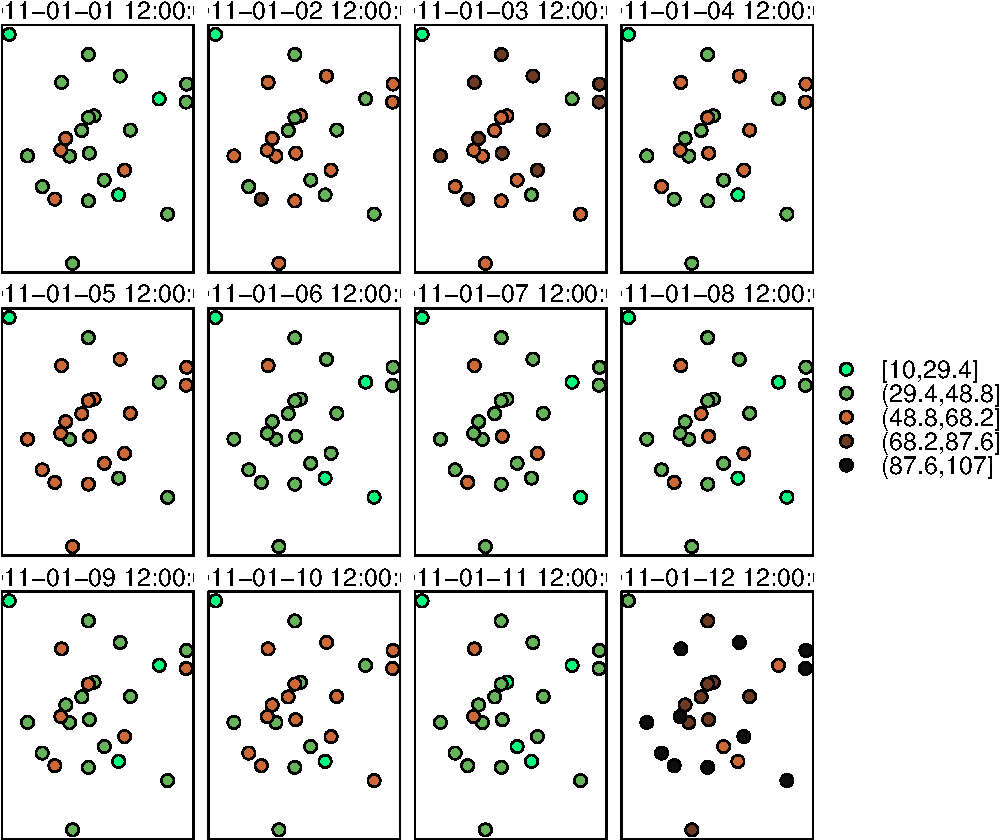
\includegraphics[width=.9\linewidth]{figs/NO2STxy.pdf}
\caption{\label{fig:NO2STxy}Scatterplots of the $NO_2$ values (2011) with a panel for each day of the time series. Each circle represents a different station.}
\end{figure}

With the mode \texttt{xt}, a space-time plot with space on the x-axis and
time on the y-axis is plotted (Figure \ref{fig:NO2hovmoller}).

\lstset{language=R,numbers=none}
\begin{lstlisting}
stplot(NO2st, mode='xt', col.regions=colorRampPalette(airPal)(15),
       scales=list(x=list(rot=45)), ylab='', xlab='')
\end{lstlisting}

\begin{figure}[htb]
\centering
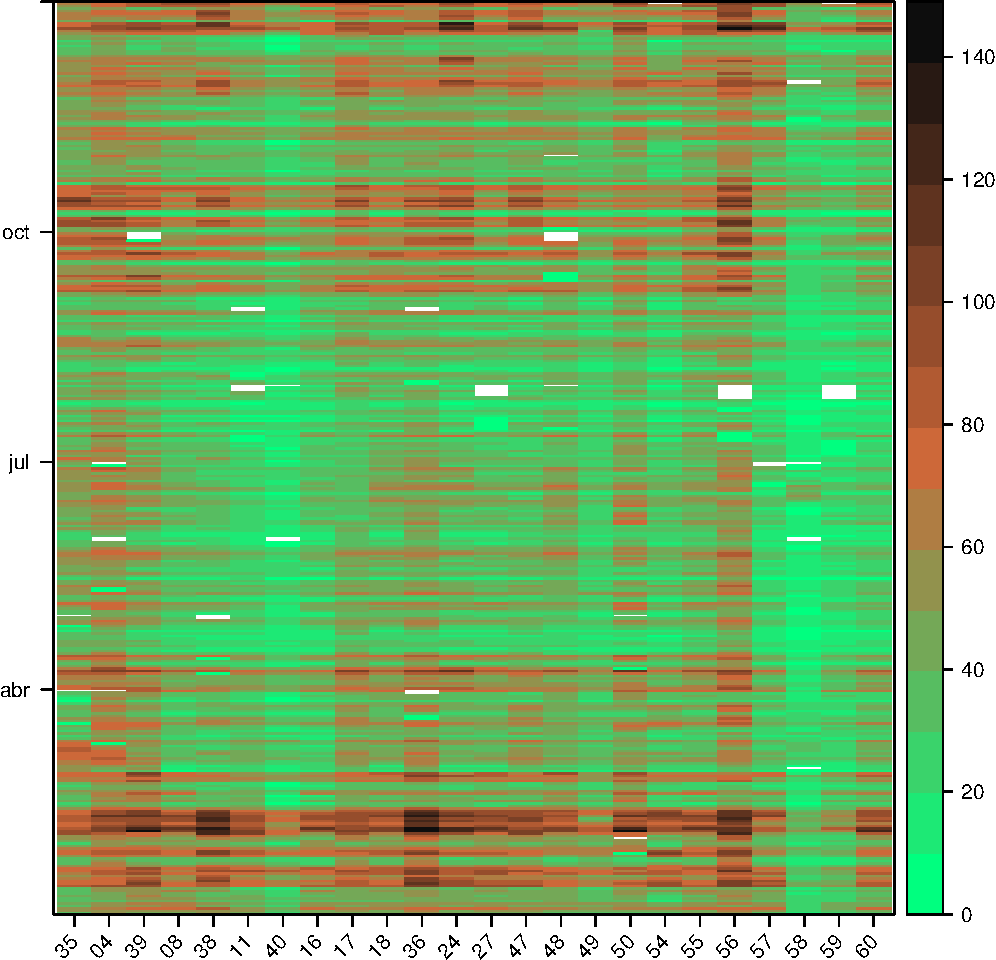
\includegraphics[width=.9\linewidth]{figs/NO2hovmoller.pdf}
\caption{\label{fig:NO2hovmoller}Space-time graphic of the NO\_2 time series. Each column represents a different station (denoted with the last two digits of the code).}
\end{figure}

Finally, with the mode \texttt{ts}, data are coerced to a multivariate time series
that is displayed in a single plot (Figure \ref{fig:NO2zoo}).

\lstset{language=R,numbers=none}
\begin{lstlisting}
stplot(NO2st, mode='ts', xlab='',
       lwd=0.1, col='black', alpha=0.6,
       auto.key=FALSE)
\end{lstlisting}

\begin{figure}[htb]
\centering
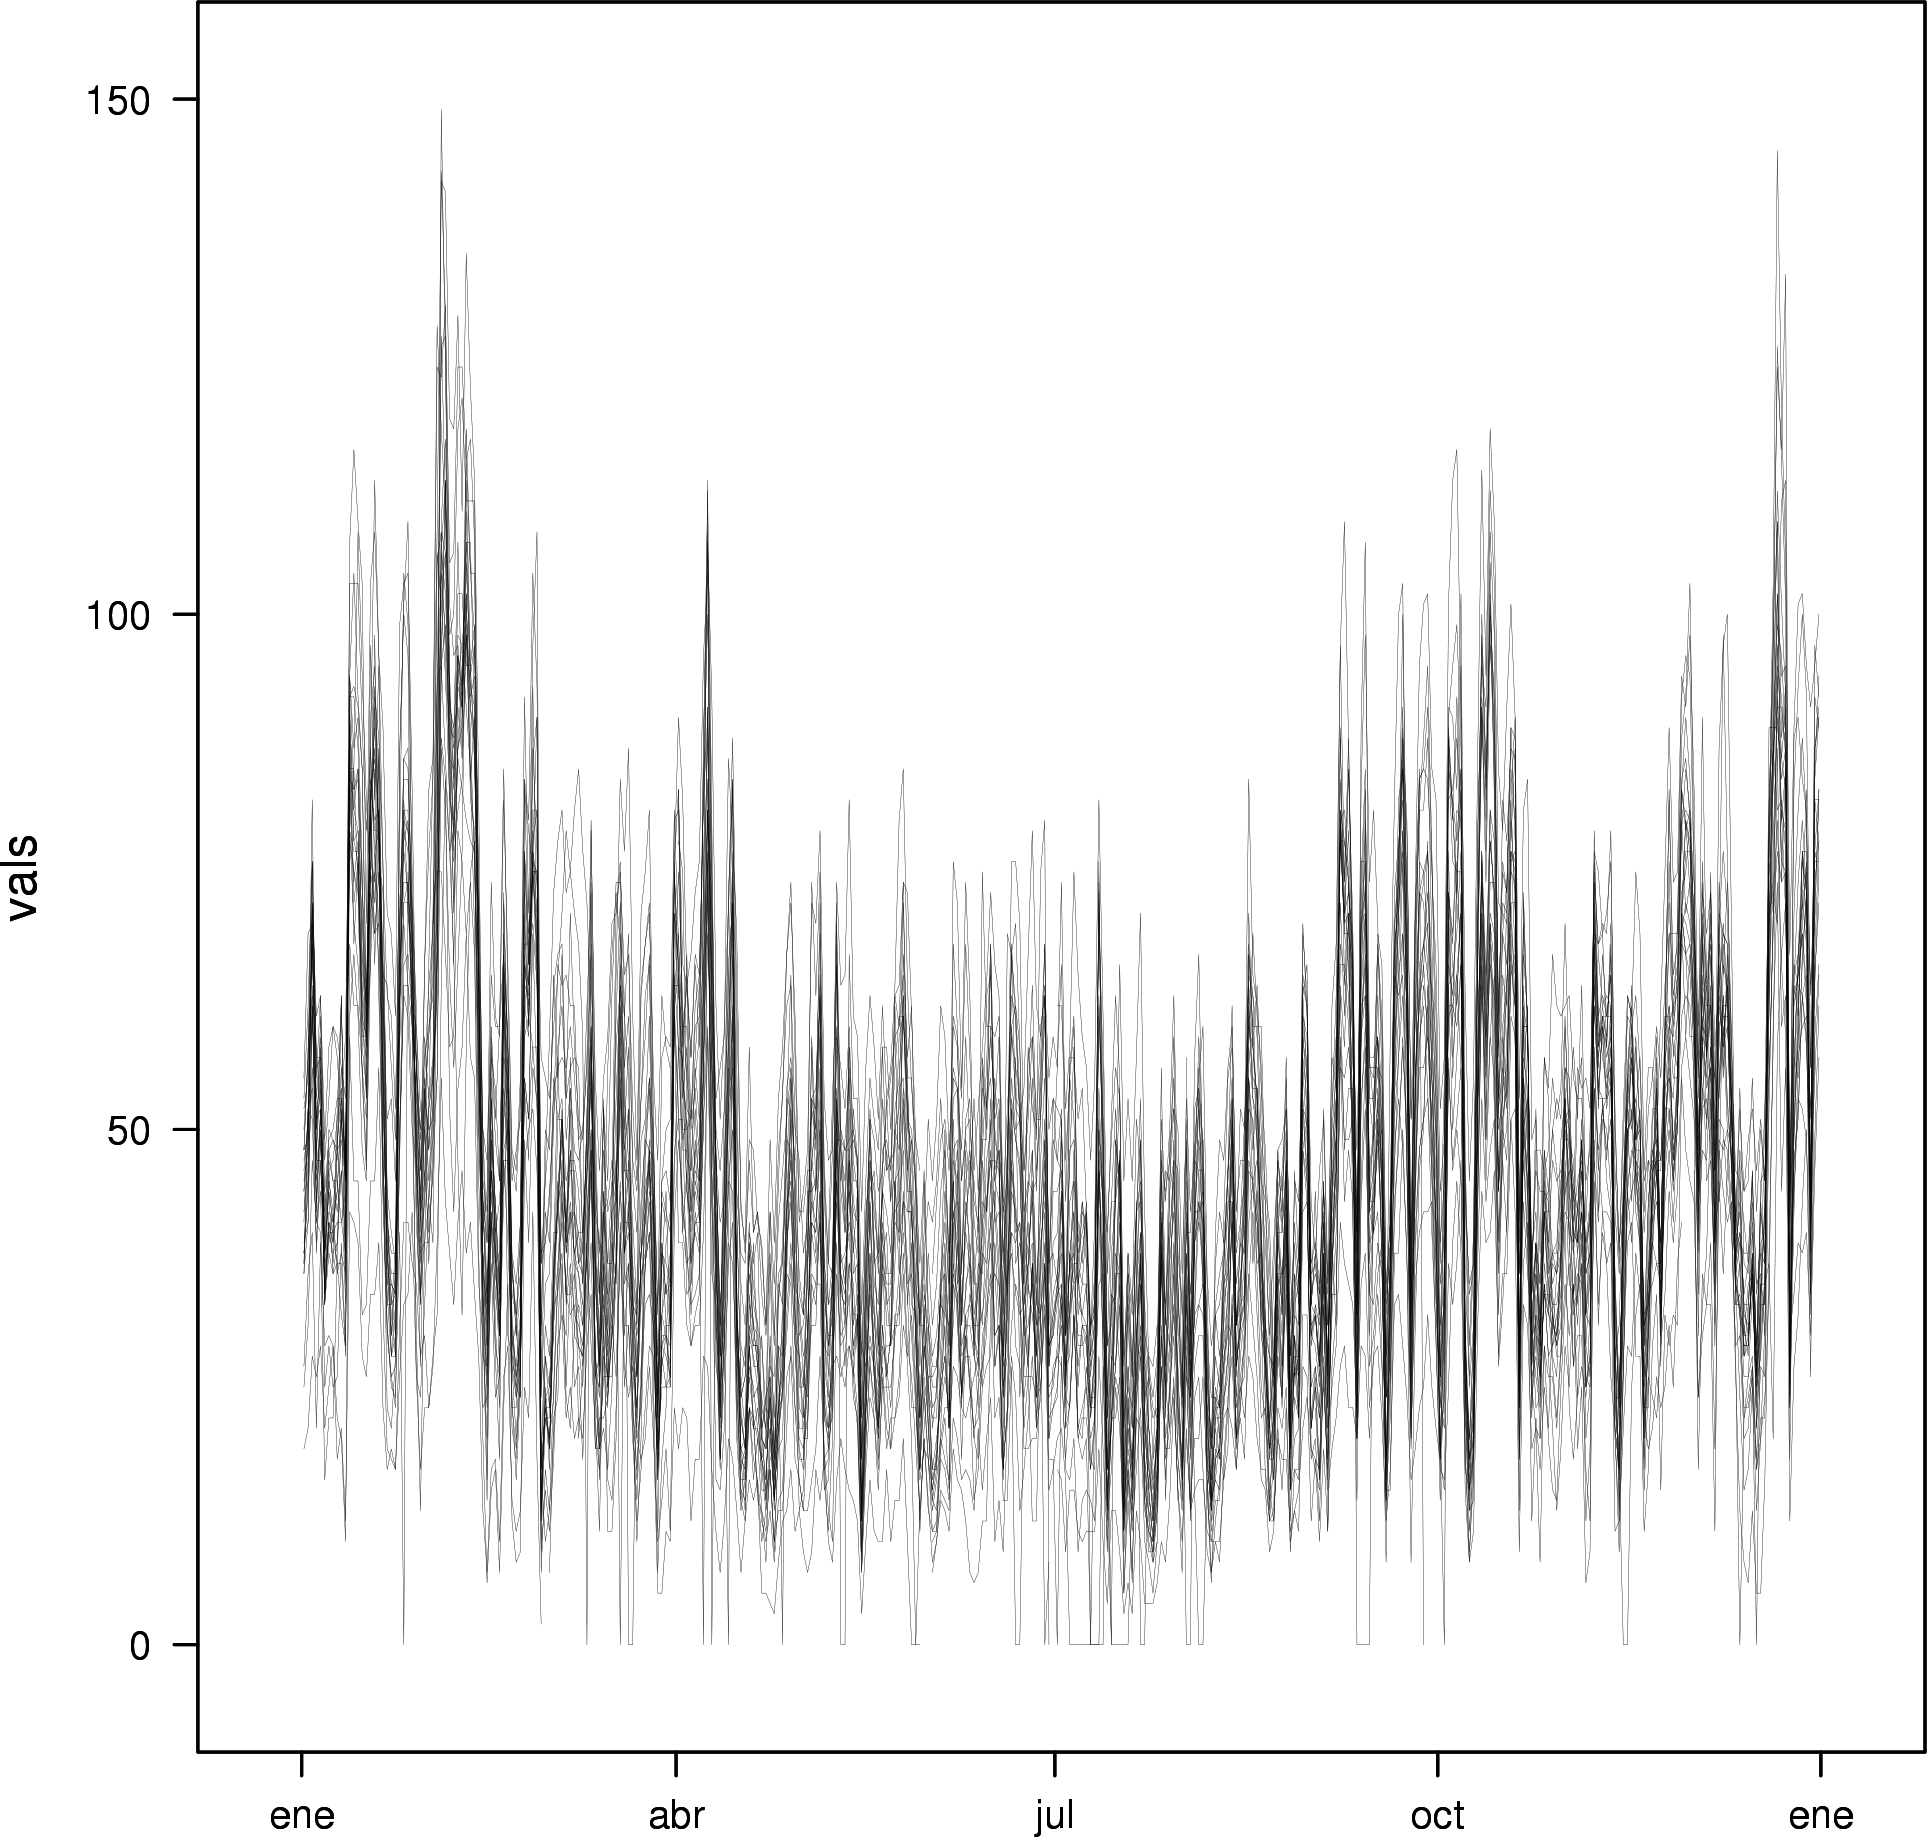
\includegraphics[width=.9\linewidth]{figs/NO2zoo.png}
\caption{\label{fig:NO2zoo}Time graph of the $NO_2$ time series (2011). Each line represents a different station.}
\end{figure}

These three graphics complement each other and together provide a more
complete view of the behavior of the data. For example in Figure
\ref{fig:NO2STxy}, we can find stations whose levels remain almost constant
throughout the 12-day period (namely, El Pardo-28079058\footnote{Use Figure \ref{fig:airMadrid} as reference of the
positions and codes of the stations.}, the
station at the top-left corner that is far from the city center),
while others fluctuate notably during this same period (for example,
Barajas-28079027 and Urb. Embajada-28079055, the two nearby stations
at the right). On the other hand, Figure \ref{fig:NO2hovmoller} loses the
spatial information but gives a more comprehensive view of the
evolution of the network. The station El Pardo-28079058 is
significantly below the rest of the stations during the whole year,
with the station Pza. Fdez Ladreda-28079056 being the opposite. In
between, the stations could be divided into two or three groups
according to their levels. Regardless, the group of stations reaches
maximum values during the first days of autumn and at the end of
winter. These maxima are clearly displayed in Figure \ref{fig:NO2zoo}.

\section{\floweroneleft Animation}
\label{sec-4}
Another approach for displaying this spatiotemporal data is using
animation. Once again, we will take advantage of the functionalities
of the \texttt{gridSVG} package.

\subsection{Initial Snapshot}
\label{sec-4-1}
The first step is to define the initial parameters of the animation:
starting values and duration.

\index{Packages!gridSVG@\texttt{gridSVG}}

\lstset{language=R,numbers=none}
\begin{lstlisting}
library(gridSVG)
## Initial parameters
start <- NO2st[,1]
## values will be encoded as size of circles,
## so we need to scale them
startVals <- start$vals/5000

nStations <- nrow(airStations)
days <- index(NO2zoo)
nDays <- length(days)
## Duration in seconds of the animation
duration <- nDays*.3
\end{lstlisting}

The first snapshot of the data is produced with \texttt{spplot}. We define an
auxiliary function, \texttt{panel.circlesplot}, to display the data encoding
values with circles of variable size and color.  This function
uses \texttt{grid.circle} from the \texttt{grid} package.  

The subsequent frames of the animation will modify the colors and
sizes of the circles according to the \texttt{NO2st} object.

\index{Packages!grid@\texttt{grid}}
\index{grid.circle@\texttt{grid.circle}}
\index{spplot@\texttt{spplot}}

\lstset{language=R,numbers=none}
\begin{lstlisting}
library(grid)

## Auxiliary panel function to display circles
panel.circlesplot <- function(x, y, cex, col='gray',
			      name='stationsCircles', ...){
grid.circle(x, y, r=cex,
	    gp=gpar(fill=col, alpha=0.5),
	    default.units='native', name=name)
}

pStart <- spplot(start, panel=panel.circlesplot,
		 cex=startVals,
		 scales=list(draw=TRUE), auto.key=FALSE)
pStart
\end{lstlisting}
\subsection{Intermediate States to Create the Animation}
\label{sec-4-2}
From this initial state, \texttt{grid.animate} creates a collection of
animated graphical objects with the intermediate states defined by
\texttt{animUnit} and \texttt{animValue}.  As previously stated, the $NO_2$ values
will be encoded with the radius of each circle, and the color of the
circles will distinguish between weekdays and weekend.  The use of
\texttt{rep=TRUE} ensures that the animation will be repeated indefinitely.

\index{animValue@\texttt{animValue}}
\index{animUnit@\texttt{animUnit}}
\index{grid.animate@\texttt{grid.animate}}

\lstset{language=R,numbers=none}
\begin{lstlisting}
## Color to distinguish between weekdays ('green')
## and weekend ('blue')
isWeekend <- function(x) {format(x, '%w') %in% c(0, 6)}
color <- ifelse(isWeekend(days), 'blue', 'green')
colorAnim <- animValue(rep(color, each=nStations),
		       id=rep(seq_len(nStations), nDays))

## Intermediate sizes of the circles
vals <- NO2st$vals/5000
vals[is.na(vals)] <- 0
radius <- animUnit(unit(vals, 'native'),
		       id=rep(seq_len(nStations), nDays))                     

## Animation of circles including sizes and colors
grid.animate('stationsCircles',
	     duration=duration,
	     r=radius,
	     fill=colorAnim,
	     rep=TRUE)
\end{lstlisting}
\subsection{Time Reference: Progress Bar}
\label{sec-4-3}
Information from an animation is better understood if a time
reference is included, for example with a progress bar.  The following
code builds a progress bar with ticks at the first day of each
month, and with color changing from gray (background) to blue as
the time advances.  On the other hand, it is convenient to provide
a method so the user can stop and restart the animation sequence
if desired.  This functionality is added with the definition of
two events, \texttt{onmouseover} and \texttt{onmouseout}, included with the
\texttt{grid.garnish} function.

\index{grid.rect@\texttt{grid.rect}}
\index{grid.text@\texttt{grid.text}}
\index{grid.animate@\texttt{grid.animate}}
\index{grid.segments@\texttt{grid.segments}}
\index{grid.garnish@\texttt{grid.garnish}}

\lstset{language=R,numbers=none}
\begin{lstlisting}
## Progress bar
prettyDays <- pretty(days, 12)
## Width of the progress bar
pbWidth <- .95
## Background
grid.rect(.5, 0.01, width=pbWidth, height=.01,
	  just=c('center', 'bottom'),
	  name='bgbar', gp=gpar(fill='gray'))

## Width of the progress bar for each day
dayWidth <- pbWidth/nDays
ticks <- c(0, cumsum(as.numeric(diff(prettyDays)))*dayWidth) + .025
grid.segments(ticks, .01, ticks, .02)
grid.text(format(prettyDays, '%d-%b'),
		 ticks, .03, gp=gpar(cex=.5))
## Initial display of the progress bar
grid.rect(.025, .01, width=0,
	  height=.01, just=c('left', 'bottom'),
	  name='pbar', gp=gpar(fill='blue', alpha='.3'))
## ...and its animation
grid.animate('pbar', duration=duration,
	     width=seq(0, pbWidth, length=duration),
	     rep=TRUE)
## Pause animations when mouse is over the progress bar
grid.garnish('bgbar',
	     onmouseover='document.rootElement.pauseAnimations()',
	     onmouseout='document.rootElement.unpauseAnimations()')
\end{lstlisting}

The SVG file is finally produced with \texttt{gridToSVG} (Figure \ref{fig:NO2pb})

\index{grid.export@\texttt{grid.export}}  

\lstset{language=R,numbers=none}
\begin{lstlisting}
grid.export('figs/NO2pb.svg')
\end{lstlisting}

\begin{figure}
  \centering
  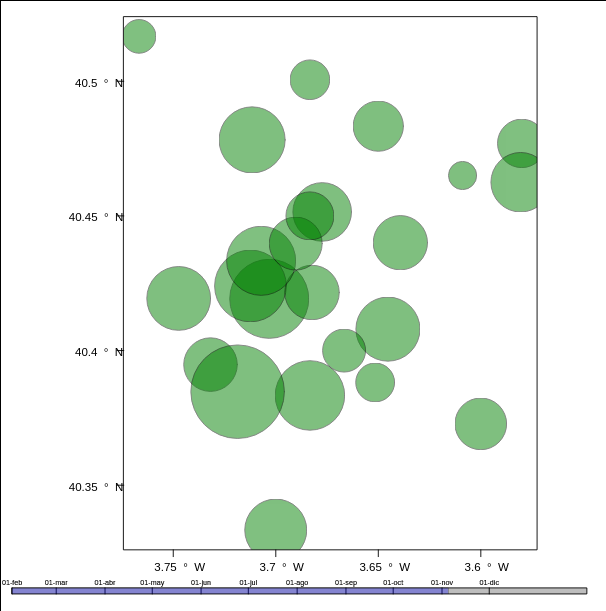
\includegraphics[width=\textwidth]{figs/NO2pb.png}
  \caption{Animated circles of the $NO_2$ space-time data with a progress bar.}
  \label{fig:NO2pb}
\end{figure}
\subsection{Time Reference: A Time Series Plot}
\label{sec-4-4}
A different and more informative solution is to add a time series
plot instead of a progress bar.  This time series plot displays
the average value of the set of stations, with a point and a
vertical line to highlight the time position as the animation
advances (Figure \ref{fig:vLine}).
\lstset{language=R,numbers=none}
\begin{lstlisting}
## Time series with average value of the set of stations
NO2mean <- zoo(rowMeans(NO2zoo, na.rm=TRUE), index(NO2zoo))
## Time series plot with position highlighted
pTimeSeries <- xyplot(NO2mean, xlab='', identifier='timePlot') +
    layer({
	grid.points(0, .5, size=unit(.5, 'char'),
		    default.units='npc',
		    gp=gpar(fill='gray'),
		    name='locator')
	grid.segments(0, 0, 0, 1, name='vLine')
    })

print(pStart, position=c(0, .2, 1, 1), more=TRUE)
print(pTimeSeries, position=c(.1, 0, .9, .25))
\end{lstlisting}


Once again, \texttt{grid.animate} creates a sequence of intermediate states
for each object of the graphical scenes: The signaling point and
vertical line follow the time evolution, while the sizes and colors of
each station circle change as in the previous approach.  Moreover, the
\texttt{onmouseover} and \texttt{onmouseout} events are defined with \texttt{grid.garnish}
so the user can pause and restart the animation by hovering the mouse
over the time series plot.
\lstset{language=R,numbers=none}
\begin{lstlisting}
grid.animate('locator',
	     x=unit(as.numeric(index(NO2zoo)), 'native'),
	     y=unit(as.numeric(NO2mean), 'native'),
	     duration=duration, rep=TRUE)

xLine <- unit(index(NO2zoo), 'native')

grid.animate('vLine',
	     x0=xLine, x1=xLine,
	     duration=duration, rep=TRUE)

grid.animate('stationsCircles',
	     duration=duration,
	     r=radius,
	     fill=colorAnim,
	     rep=TRUE)

## Pause animations when mouse is over the time series plot
grid.garnish('timePlot', grep=TRUE,
	     onmouseover='document.rootElement.pauseAnimations()',
	     onmouseout='document.rootElement.unpauseAnimations()')

grid.export('figs/vLine.svg')
\end{lstlisting}


\begin{figure}
  \centering
  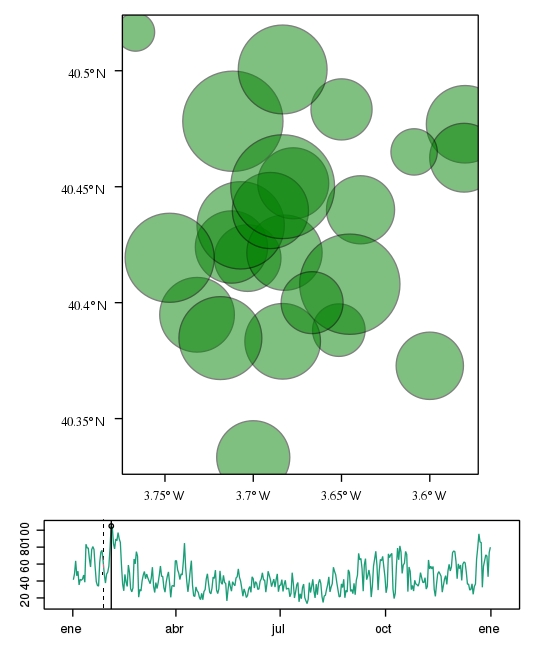
\includegraphics[width=\textwidth]{figs/vLine.png}
  \caption{Animated circles of the $NO_2$ space-time data with a a time series as reference.}
  \label{fig:vLine}
\end{figure}
